\documentclass[slovene,11pt,a4paper]{article}
%\usepackage{fullpage}
\usepackage[margin=2cm]{geometry}

\usepackage[T1]{fontenc}



%dodatni paketki:
\usepackage{graphicx}
\usepackage{amsmath,amsfonts,amsthm} %matematicni paket
\usepackage{color} % omogoča barvno pisanje
\usepackage[utf8]
{inputenc}
\usepackage[slovene]{babel} % slovenski jezik/hyphenation
\usepackage{hyperref} %naredi vse povezave rečerenc, kazala,...
\numberwithin{equation}{section} % Number equations within sections (i.e. 1.1, 1.2, 2.1, 2.2 instead of 1, 2, 3, 4)
\numberwithin{figure}{section} % Number figures within sections (i.e. 1.1, 1.2, 2.1, 2.2 instead of 1, 2, 3, 4)
\numberwithin{table}{section} % Number tables within sections (i.e. 1.1, 1.2, 2.1, 2.2 instead of 1, 2, 3, 4)
\usepackage{eurosym} %za znak €

\usepackage{mathrsfs}
\usepackage{mathabx} % za kemisjke smeri in naslednje 3 vstrice
\catcode`_=12
\begingroup\lccode`~=`_\lowercase{\endgroup\let~\sb}
\mathcode`_="8000


\usepackage[margin=2cm]{geometry}



\begin{document}
\begin{titlepage}

\newcommand{\HRule}{\rule{\linewidth}{0.5mm}} % Defines a new command for the horizontal lines, change thickness here

\center % Center everything on the page

%----------------------------------------------------------------------------------------
%	LOGO
%----------------------------------------------------------------------------------------

%\includegraphics{Logo}\\[1cm] % Include a department/university logo - this will require the graphicx package
 
%----------------------------------------------------------------------------------------


\includegraphics[width=2cm]{slike/aaa}\\[0.5cm]
 
%----------------------------------------------------------------------------------------
%	NASLOV DELA
%----------------------------------------------------------------------------------------
\textit{Univerza v Ljubljani}\\
\textit{Fakulteta za {\color{red}matematiko in fiziko}}\\[0.5cm]

\emph{Oddelek za fiziko}\\[0.5cm] % Oddelek za fiziko


%----------------------------------------------------------------------------------------
%	TITLE SECTION
%--------------------------------------------------------------------------------------
\HRule \\[0.4cm]
\huge {\bfseries 9. naloga: - Integracije z metodo Monte Carlo}\\[0.4cm] % NASLOV SEMINARJA
\HRule \\[0.5cm] 

 \textsc{\large Poročilo pri predmetu modelska analiza 1}\\
 \textsc{\large 2015/2016}\\[1cm] % SEMINASKO DELO
 
%----------------------------------------------------------------------------------------
%	AUTHOR SECTION
%----------------------------------------------------------------------------------------



% If you don't want a supervisor, uncomment the two lines below and remove the section above
\Large \emph{Avtor:}\\
Klemen \textsc{Rahne}\\
28152028\\[2cm]
%----------------------------------------------------------------------------------------
%	DATUM
%----------------------------------------------------------------------------------------

{\large \today } \\[0.5cm] % Date, change the \today to a set date if you want to be precise

	

\end{titlepage}


%----------------------------------------------------------------------------------------
%	KAZALO
%----------------------------------------------------------------------------------------

%\tableofcontents

%----------------------------------------------------------------------------------------
%	ZAČETEK TEKSTA
%----------------------------------------------------------------------------------------


\section{Izrezana krogla}
Imamo kroglo z radijem $R=1$, kateri izrežemo valj, s središčem v $(\frac{1}{2},0,z)$ in radijem $R=\frac{1}{2}$. Naša naloga je izračunati maso in težišče omenjenega objekta s pomočjo metode Monte Carlo. 
Pri metodi Monte Carlo za izračunanje integrala generiramo naključne točke v izbranem prostoru. V našem primeru bomo generirali $N$ točk v krogli z radijem $r=1$:
\begin{equation}
\begin{aligned}
r=& (\xi_1)^{\frac{1}{3}} \\
\phi=& 2 \pi \xi_2 \\
\theta = & \arccos(2 \xi_3 -1)
\end{aligned}
\end{equation}
kjer so $\xi_1$, $\xi_2$ in $\xi_3$ porazdeljene uniformno med $0$ in $1$. V primeru, da bo posamezna točka v valju, oz. izpolnjevala:
\begin{equation}
(x-\frac{1}{2})^2 +y^2 \leq R^2=\frac{1}{4}
\end{equation}
bomo točko zavrgli, saj ni v našem telesu.

\begin{figure}[h]
\begin{center}

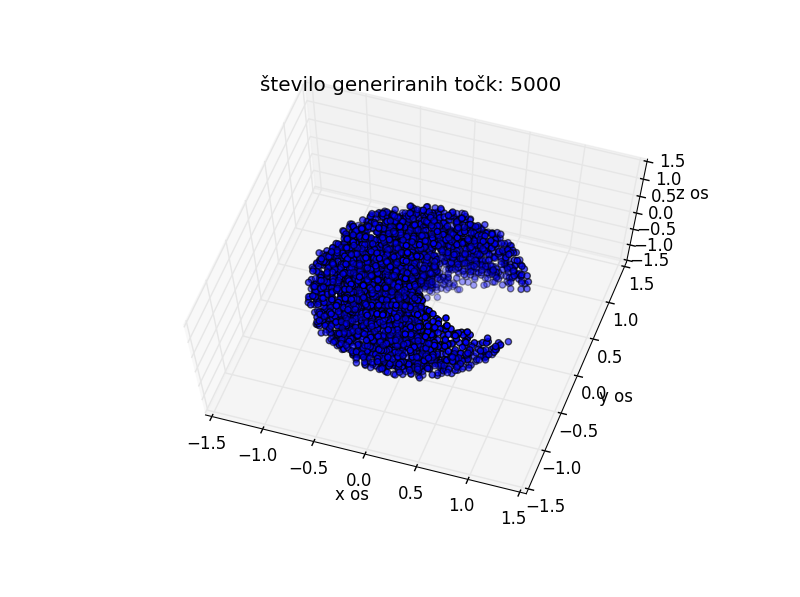
\includegraphics[scale=0.7]{slike/prva_objekt.png}

\caption{$5000$ generiranih točk v krogli ter  $3489$ točk znotraj našega objekta.}
\end{center}
\end{figure}

Maso telesa se analitično izračuna kot integral gostote po volumnu, ker pa je v našem primeru gostota konstanta (v brezdimezijska obliki je gostota enaka $1$):
\begin{equation}
m= \int \rho dV = \int dV
\end{equation}
Torej je treba le izračunati volumen objekta. Volumen objekta bomo izračunali preko razmerja vseh izbranih točk in točk, ki so v našem telesu:
\begin{equation}
\frac{N_{nezavrženih}}{N}=\frac{V_{telesa}}{V_{krogle}}=\frac{3 V_{telesa}}{4 \pi}
\end{equation}
Od to sledi:
\begin{equation}
V_{telesa}=\frac{N_{nezavrzenih }4 \pi}{ N 3}
\end{equation}
Težišče objekta se analitično izračuna:
\begin{equation}
\label{masa-tezisce}
\begin{aligned}
x_T=& \frac{1}{m}\int_V x \rho dV = \frac{1}{m}\int_V x dV \\
y_T =& \frac{1}{m}\int_V y \rho dV =\frac{1}{m}\int_V y dV \\
z_T =& \frac{1}{m}\int_V z \rho dV =\frac{1}{m}\int_V z dV
\end{aligned}
\end{equation}
pri metodi Monte Carlo se zgornji integrali prepišejo v:
\begin{equation}
x_T=\frac{1}{N} \sum_i^N x_i 
\end{equation}
za $y_T$ in $z_T$ je podoben zapis.
Rešitve po tej metodi so:
\begin{table}[h]
\begin{center}
\begin{tabular}{|l|l|l|l|}
\hline
masa & $x_T$ & $y_T$ & $z_T$ \\ \hline
$2.9229$ & $-0.1789$ & $0.0029$ & $-0.0018$ \\ \hline

\end{tabular}
\end{center}
\end{table}


\subsection{Nekonstanta gostota}
V zgornjem primeru smo obravnavali konstantno gostoto. Predpostavimo, da ima naša prvotna krogla pred izrezom valja gostoto, kot funkcijo razdalje:
\begin{equation}
\rho = \rho_0 r^3
\end{equation}
Torej kot v prejšnjem poglavju so za maso in težišče enačbe \ref{masa-tezisce} podobne, le da se zaradi odvisnosti gostote malenkost spremenijo:

\begin{equation}
\begin{aligned}
m=&\int r^3 dV \\
x_T=&\frac{1}{m}\int_V x r^3 dV \\
y_T =& \frac{1}{m}\int_V y r^3 dV \\
z_T =& \frac{1}{m}\int_V z r^3 dV
\end{aligned}
\end{equation}
Za reševenje omenjenih integralov lahko uporabimo točke iz zgornje naloge, z ustrezno utežjo ($r^3$) ali pa točke v našem objektu ponovno generiramo s upoštevanjem uteži ($r^3$).
Odločil sem se za uporabo slednje metode in samo radialni del točk generiral:
\begin{equation}
r=\xi^{\frac{1}{6}}
\end{equation}
kjer je $\xi$ porazdeljen uniformno med $0$ in $1$. Ostala kotna dela sta porazdeljena enako kot v prejšnji nalogi, saj se ta del ni nič spreminjal.
Sedaj smo prišli do rešitev:
\begin{table}[h]
\begin{center}
\begin{tabular}{|l|l|l|l|}
\hline
masa & $x_T$ & $y_T$ & $z_T$ \\ \hline
$3.1441$ & $-0.1854$ & $0.0014$ & $-4.3*10^{-5}$ \\ \hline
\end{tabular}
\end{center}
\end{table}

\pagebreak
\section{Sevanje žarkov gama v krogli}
Imamo kroglo, v kateri je izvor žarkov gama enakomerno porazdeljen po krogli. Ko se žarek izseva, potuje skozi snov v krogli, pri čemer se lahko ponovno absorbira. Naša naloga je izračunati delež izsevanih fotonov odvisnosti od povprečne proste poti fotona v krogli.\\
Porazdelitev proste poti fotonov v snovi je:
\begin{equation}
l=-\lambda \ln(1-\xi )
\end{equation}
kjer je $\xi$ porazdeljen uniformno med $0$ in $1$ ter $\lambda$ povprečna prosta pot v snovi. Ali se bo rojen foton v krogli izsevan izven krogle je odvisno sedaj, kje v krogli se je rodil in v katero smer se bo izseval. Če bo predlagana prosta pot za dan foton ($l$) večja kot dolžina poti, ki jo foton potrebuje za izhod iz krogle ($d$) večja, potem se bo foton izseval, v nasprotnem primeru pa se bo v krogli absorbiral. Kakšna je sedaj dolžina poti, ki jo foton potrebuje za izhod iz krogle? Zaradi simetrije problema (krogla) je potrebno za posamezni foton dovolj, če povemo radij ($r$), na katerem se je rodil, in smer v katero se bo izseval ($\theta$). Radij roditve in smer fotona sta porazdeljena:
\begin{equation}
\begin{aligned}
r=&(\xi_1)^{\frac{1}{3}} \\
\cos \theta =&t = 2 \xi_2 -1
\end{aligned}
\end{equation}
kjer sta $\xi_1$ in $\xi_2$ porazdeljena enakomerna med $0$ in $1$. Dolžina poti potrebna za izhod iz krogle za posamični foton je:
\begin{equation}
d_i=-r_i t_i+\sqrt{1-r_i^2(1-t_i^2)}
\end{equation}
Podobno kot pri računanju mase/volumna objekta pri prejšnji nalogi, za prepuščeni foton štejemo, če je njegova prosta pot večja od dolžine za izhod iz krogle. Na koncu preštejemo vse izsevane fotone in delimo z število vseh rojenih fotonov.



\begin{figure}[h]
\begin{center}

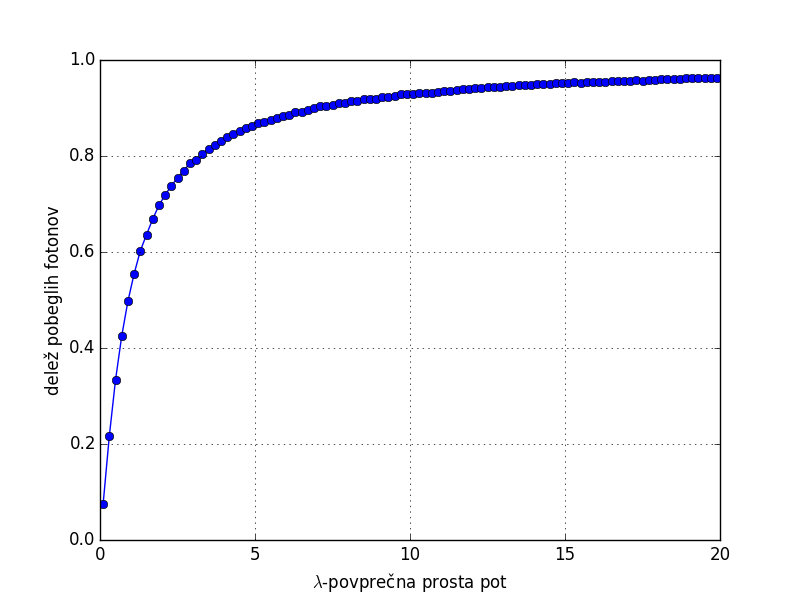
\includegraphics[scale=0.65]{slike/9_druga.png}

\caption{Delež pobeglih fotonov pri $100000$ generiranih fotonih, radij krogle je $1$. Opazimo hitro naraščanje deleža vseh fotonov proti $1$. To je posledica tega, da je pri velikih povprečnih prostih poteh doseg fotona velik, ter ne čuti ovire.}
\end{center}
\end{figure}

\section{Nevtronski reflektor}
Imamo ploščo, debeline $d$, na katero vpada tok  nevtronov. V plošči se nevtroni samo sipljejo in nič absorbirajo. Med seboj bomo primerjali dva modela: ko se fotoni sipljejo le naprej in nazaj (z enako verjetnostjo za naprej in nazaj) ter, ko se fotoni sipljejo izotropno po prostoru.
Najprej generirajmo proste poti za posamezne nevtrone. Enako, kot za fotone velja:
\begin{equation}
l=-\lambda \ln(1-\xi )
\end{equation}
V primeru, ko je je $l$ večji od debeline plošče, je plošča prepustila nevtron. Če je $l$ manjši kot debelina plasti, je potrebno sipanemu nevtronu določiti novo prosto pot, ter v primeru sipanja naprej/nazaj še smer. V anizotropnem primeru, mu določimo smer $\theta$, ter nato novo prosto pot določimo s projekcijo proste poti na os vpadnih nevtronov. Nato k sedanjemu položaju sipanja prištejemo/odštejemo novo prosto pot. V obeh primerih, ko položaj naslednjega sipanja zapusti plast plošče se nevtron ali odbije ali prepusti.

\begin{figure}[h]
\noindent\makebox[\textwidth][l]{%
\hspace{-\dimexpr\oddsidemargin+1in}%

\begin{minipage}[t]{0.5\paperwidth}
\begin{flushleft}

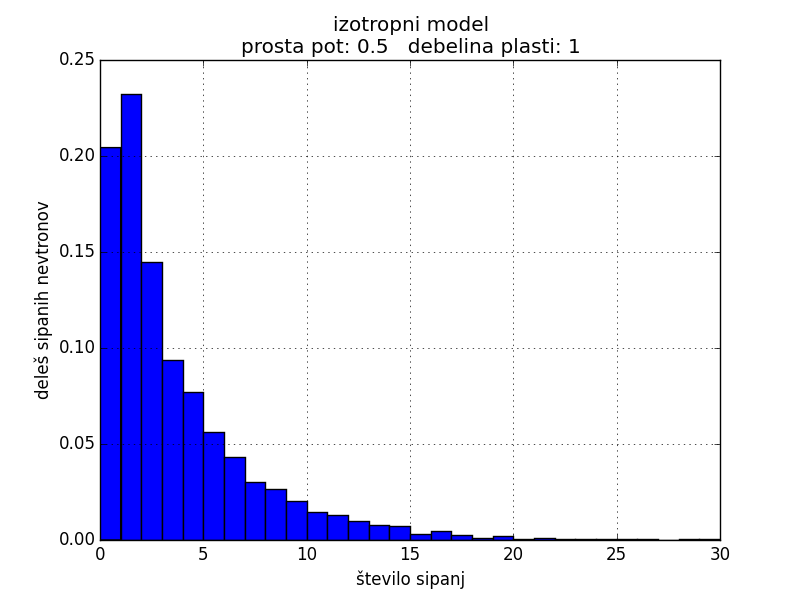
\includegraphics[scale=0.45]{slike/9_3_izotropni.png}
%\caption{Nelinearno prilagajanje $I=I_0 [\exp{\frac{U}{U_a}}- \exp{-\frac{U}{U_b}}]$.}
\hspace{\fill}
\end{flushleft}
\end{minipage}
\begin{minipage}[t]{0.5\paperwidth}
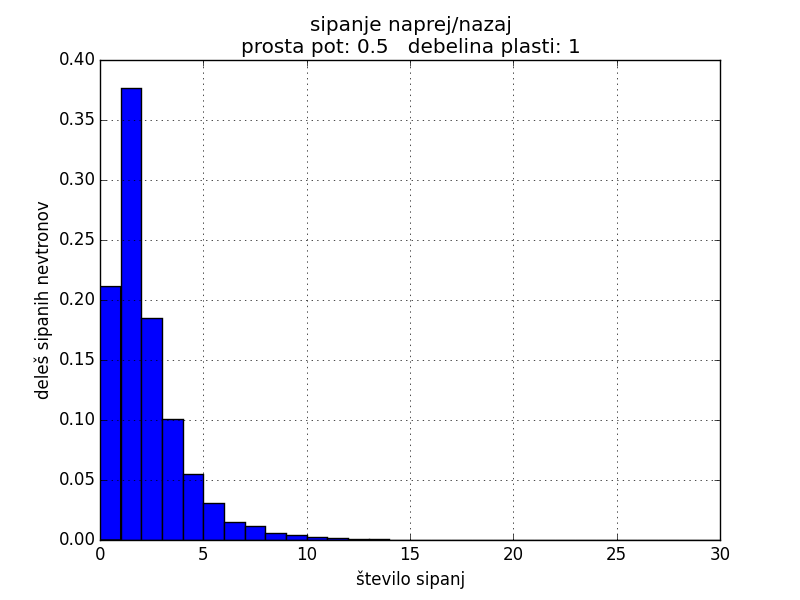
\includegraphics[scale=0.45]{slike/9_3_naprej.png}
%\caption{Nelinearno prilagajanje s premikom napetosti.}
\end{minipage}%
}
\caption{Primerjava med modeloma. Opazimo, podobno obliko. Razlika nastopa v skali. Pri izotropnem modelu imamo večji delež vsaj enkrat sipanih nevtronov, kar je najverjetneje posledica tega, da smo z vpeljavo smernega sipanja povečali efektivno debelino plasti. Število nevtronov v curku je $10000$.}
\end{figure}

\begin{figure}[t]
\begin{center}
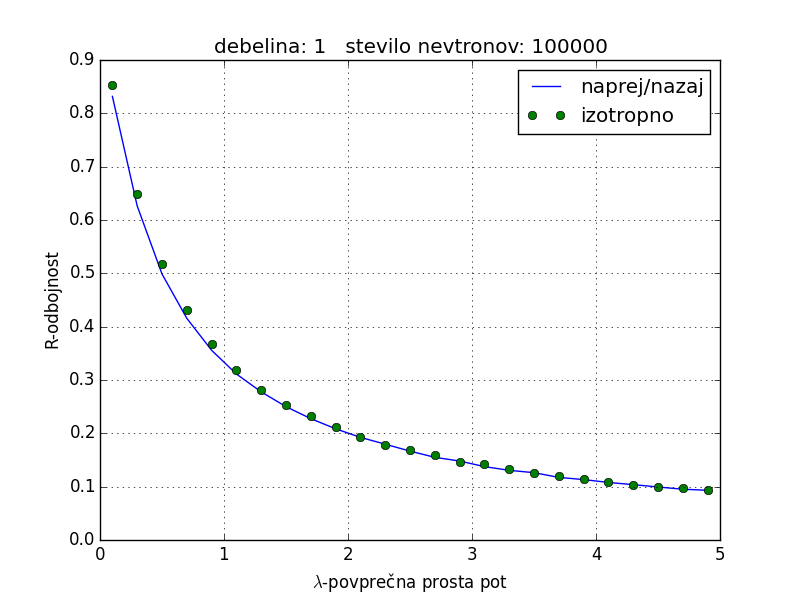
\includegraphics[scale=0.65]{slike/9_3_lamda.png}
\caption{Primerjava obeh modelov pri različnih vrednosti povprečne proste poti za nevtrone v plošči. Opazimo da se modela v sami odbojnosti zelo malo razlikujeta. Opazimo da pri majhnih prostih poteh se vsi nevtroni odbijejo, saj v tem primeru plošča deluje kot neskončno debela plošča in ne prepusti nobenega nevtrona.}
\end{center}
\end{figure}



\pagebreak
%-----------------------------------------------------------------------------

















\end{document}
